% Options for packages loaded elsewhere
\PassOptionsToPackage{unicode}{hyperref}
\PassOptionsToPackage{hyphens}{url}
%
\documentclass[
]{book}
\title{설치형 오픈 통계 패키지 - \texttt{Rcmdr}}
\author{신종화, 이광춘, 유충현, 홍성학}
\date{2022-04-16}

\usepackage{amsmath,amssymb}
\usepackage{lmodern}
\usepackage{iftex}
\ifPDFTeX
  \usepackage[T1]{fontenc}
  \usepackage[utf8]{inputenc}
  \usepackage{textcomp} % provide euro and other symbols
\else % if luatex or xetex
  \usepackage{unicode-math}
  \defaultfontfeatures{Scale=MatchLowercase}
  \defaultfontfeatures[\rmfamily]{Ligatures=TeX,Scale=1}
\fi
% Use upquote if available, for straight quotes in verbatim environments
\IfFileExists{upquote.sty}{\usepackage{upquote}}{}
\IfFileExists{microtype.sty}{% use microtype if available
  \usepackage[]{microtype}
  \UseMicrotypeSet[protrusion]{basicmath} % disable protrusion for tt fonts
}{}
\makeatletter
\@ifundefined{KOMAClassName}{% if non-KOMA class
  \IfFileExists{parskip.sty}{%
    \usepackage{parskip}
  }{% else
    \setlength{\parindent}{0pt}
    \setlength{\parskip}{6pt plus 2pt minus 1pt}}
}{% if KOMA class
  \KOMAoptions{parskip=half}}
\makeatother
\usepackage{xcolor}
\IfFileExists{xurl.sty}{\usepackage{xurl}}{} % add URL line breaks if available
\IfFileExists{bookmark.sty}{\usepackage{bookmark}}{\usepackage{hyperref}}
\hypersetup{
  pdftitle={설치형 오픈 통계 패키지 - Rcmdr},
  pdfauthor={신종화, 이광춘, 유충현, 홍성학},
  hidelinks,
  pdfcreator={LaTeX via pandoc}}
\urlstyle{same} % disable monospaced font for URLs
\usepackage{color}
\usepackage{fancyvrb}
\newcommand{\VerbBar}{|}
\newcommand{\VERB}{\Verb[commandchars=\\\{\}]}
\DefineVerbatimEnvironment{Highlighting}{Verbatim}{commandchars=\\\{\}}
% Add ',fontsize=\small' for more characters per line
\usepackage{framed}
\definecolor{shadecolor}{RGB}{248,248,248}
\newenvironment{Shaded}{\begin{snugshade}}{\end{snugshade}}
\newcommand{\AlertTok}[1]{\textcolor[rgb]{0.94,0.16,0.16}{#1}}
\newcommand{\AnnotationTok}[1]{\textcolor[rgb]{0.56,0.35,0.01}{\textbf{\textit{#1}}}}
\newcommand{\AttributeTok}[1]{\textcolor[rgb]{0.77,0.63,0.00}{#1}}
\newcommand{\BaseNTok}[1]{\textcolor[rgb]{0.00,0.00,0.81}{#1}}
\newcommand{\BuiltInTok}[1]{#1}
\newcommand{\CharTok}[1]{\textcolor[rgb]{0.31,0.60,0.02}{#1}}
\newcommand{\CommentTok}[1]{\textcolor[rgb]{0.56,0.35,0.01}{\textit{#1}}}
\newcommand{\CommentVarTok}[1]{\textcolor[rgb]{0.56,0.35,0.01}{\textbf{\textit{#1}}}}
\newcommand{\ConstantTok}[1]{\textcolor[rgb]{0.00,0.00,0.00}{#1}}
\newcommand{\ControlFlowTok}[1]{\textcolor[rgb]{0.13,0.29,0.53}{\textbf{#1}}}
\newcommand{\DataTypeTok}[1]{\textcolor[rgb]{0.13,0.29,0.53}{#1}}
\newcommand{\DecValTok}[1]{\textcolor[rgb]{0.00,0.00,0.81}{#1}}
\newcommand{\DocumentationTok}[1]{\textcolor[rgb]{0.56,0.35,0.01}{\textbf{\textit{#1}}}}
\newcommand{\ErrorTok}[1]{\textcolor[rgb]{0.64,0.00,0.00}{\textbf{#1}}}
\newcommand{\ExtensionTok}[1]{#1}
\newcommand{\FloatTok}[1]{\textcolor[rgb]{0.00,0.00,0.81}{#1}}
\newcommand{\FunctionTok}[1]{\textcolor[rgb]{0.00,0.00,0.00}{#1}}
\newcommand{\ImportTok}[1]{#1}
\newcommand{\InformationTok}[1]{\textcolor[rgb]{0.56,0.35,0.01}{\textbf{\textit{#1}}}}
\newcommand{\KeywordTok}[1]{\textcolor[rgb]{0.13,0.29,0.53}{\textbf{#1}}}
\newcommand{\NormalTok}[1]{#1}
\newcommand{\OperatorTok}[1]{\textcolor[rgb]{0.81,0.36,0.00}{\textbf{#1}}}
\newcommand{\OtherTok}[1]{\textcolor[rgb]{0.56,0.35,0.01}{#1}}
\newcommand{\PreprocessorTok}[1]{\textcolor[rgb]{0.56,0.35,0.01}{\textit{#1}}}
\newcommand{\RegionMarkerTok}[1]{#1}
\newcommand{\SpecialCharTok}[1]{\textcolor[rgb]{0.00,0.00,0.00}{#1}}
\newcommand{\SpecialStringTok}[1]{\textcolor[rgb]{0.31,0.60,0.02}{#1}}
\newcommand{\StringTok}[1]{\textcolor[rgb]{0.31,0.60,0.02}{#1}}
\newcommand{\VariableTok}[1]{\textcolor[rgb]{0.00,0.00,0.00}{#1}}
\newcommand{\VerbatimStringTok}[1]{\textcolor[rgb]{0.31,0.60,0.02}{#1}}
\newcommand{\WarningTok}[1]{\textcolor[rgb]{0.56,0.35,0.01}{\textbf{\textit{#1}}}}
\usepackage{longtable,booktabs,array}
\usepackage{calc} % for calculating minipage widths
% Correct order of tables after \paragraph or \subparagraph
\usepackage{etoolbox}
\makeatletter
\patchcmd\longtable{\par}{\if@noskipsec\mbox{}\fi\par}{}{}
\makeatother
% Allow footnotes in longtable head/foot
\IfFileExists{footnotehyper.sty}{\usepackage{footnotehyper}}{\usepackage{footnote}}
\makesavenoteenv{longtable}
\usepackage{graphicx}
\makeatletter
\def\maxwidth{\ifdim\Gin@nat@width>\linewidth\linewidth\else\Gin@nat@width\fi}
\def\maxheight{\ifdim\Gin@nat@height>\textheight\textheight\else\Gin@nat@height\fi}
\makeatother
% Scale images if necessary, so that they will not overflow the page
% margins by default, and it is still possible to overwrite the defaults
% using explicit options in \includegraphics[width, height, ...]{}
\setkeys{Gin}{width=\maxwidth,height=\maxheight,keepaspectratio}
% Set default figure placement to htbp
\makeatletter
\def\fps@figure{htbp}
\makeatother
\setlength{\emergencystretch}{3em} % prevent overfull lines
\providecommand{\tightlist}{%
  \setlength{\itemsep}{0pt}\setlength{\parskip}{0pt}}
\setcounter{secnumdepth}{5}
\usepackage{booktabs}
\usepackage{amsthm}
\makeatletter
\def\thm@space@setup{%
  \thm@preskip=8pt plus 2pt minus 4pt
  \thm@postskip=\thm@preskip
}
\makeatother
\ifLuaTeX
  \usepackage{selnolig}  % disable illegal ligatures
\fi
\usepackage[]{natbib}
\bibliographystyle{apalike}

\begin{document}
\maketitle

{
\setcounter{tocdepth}{1}
\tableofcontents
}
\hypertarget{uxb4e4uxc5b4uxac00uxba70}{%
\chapter{들어가며}\label{uxb4e4uxc5b4uxac00uxba70}}

\textbf{한국 알(R) 사용자회}는 디지털 불평등 해소와 통계 대중화를 오픈 통계 패키지 개발을 2021년부터 추진하였습니다.
더불어 설치형 오픈 통계 패키지를 신종화 님께서 John Fox 교수님이 개발한 \texttt{Rcmdr} 기반으로 한글화 및 문서화에 10년 넘게 기여해주셨습니다. 이에 \textbf{한국 알(R) 사용자회}는 신종화님의 \texttt{Rcmdr} 거인의 어깨위에 디지털 불평등 해소와 통계 대중화를 위해 한 걸음 더 나아가게 되었습니다. 특히 신종화님께서 기여하신 한글화 및 문서를 근간으로 더 많은 분들이 오픈 통계 패키지를 사용할 수 있도록 \texttt{bookdown}으로 내용을 정리하여 통계 대중화가 한층 앞당겨질 것으로 기대됩니다.

신종화님께서 왜 오픈 통계 패키지로 \texttt{Rcmdr}를 근간으로 해야 하는지 이유를 명쾌하게 다음과 같이 정리해 주셨습니다.

R에는 여러 개의 GUI 작업도구들이 있습니다. 모두 목적이 분명하고, 좋은 도구이며, 일부는 현재도 향상작업이 진행되고 있습니다. 그럼에도 불구하고 R Commander를 위한 블로그 작업을 진행하는 이유는 크게 두가지 입니다.

첫째, R Commander는 직관적으로 기존의 기초통계학 도구와 유사합니다. Command Line 에서 작업하는 것에 익숙하지 않은, 또 어려움을 겪고 있는 사용자들에게 기초통계학분야를 학습하고 활용하는데 도움을 주기 위하여 R Commander가 개발되었습니다. 개발자인 John Fox 교수는 이 목적과 관리방향을 분명히하고 있습니다. 중급이상의 R 사용자/ 고급통계 연구자들에게는 R Commander가 불필요할 수 있습니다.

둘째, 지난 10년동안 R Commander의 메뉴 한글화작업을 진행해왔으며, 현재도 유지관리를 하고 있습니다. (이 정보는 R Commander 안의 Help \textgreater{} About Rcmdr 에 있습니다) {[}Translations: Korean, Chel Hee Lee, Dae-Heung Jang, and Shin Jong-Hwa{]} 지난 10년 동안 개인적인 메모 차원에서 R Commander 사용 및 한글화 관련 블로그 포스트를 만들고 관리되어 왔고 \href{http://modernity.tistory.com}{블로그}에 전체 과정이 고스란히 남아있고 계속적으로 유지관리될 것입니다.

\begin{itemize}
\tightlist
\item
  신종화 \href{https://rcmdr.kr/}{Rcmdr : R Commander}
\item
  \href{https://cran.r-project.org/web/packages/Rcmdr/index.html}{CRAN Rcmdr 패키지 정보}
\item
  \href{https://socialsciences.mcmaster.ca/jfox/Misc/Rcmdr/}{개발자 John Fox 교수의 Rcmdr 소개}
\item
  \href{https://modernity.tistory.com/}{FOSSER\_Ricoop}
\end{itemize}

\hypertarget{install}{%
\chapter{설치}\label{install}}

\hypertarget{tools}{%
\chapter{Tools}\label{tools}}

\hypertarget{uxb3c4uxad6c-uxd328uxd0a4uxc9c0-uxc801uxc7acuxd558uxae30}{%
\section{도구 \textgreater{} 패키지 적재하기\ldots{}}\label{uxb3c4uxad6c-uxd328uxd0a4uxc9c0-uxc801uxc7acuxd558uxae30}}

\texttt{도구\ \textgreater{}\ 패키지\ 적재하기...\ /\ Tools\ \textgreater{}\ Load\ package(s)...}

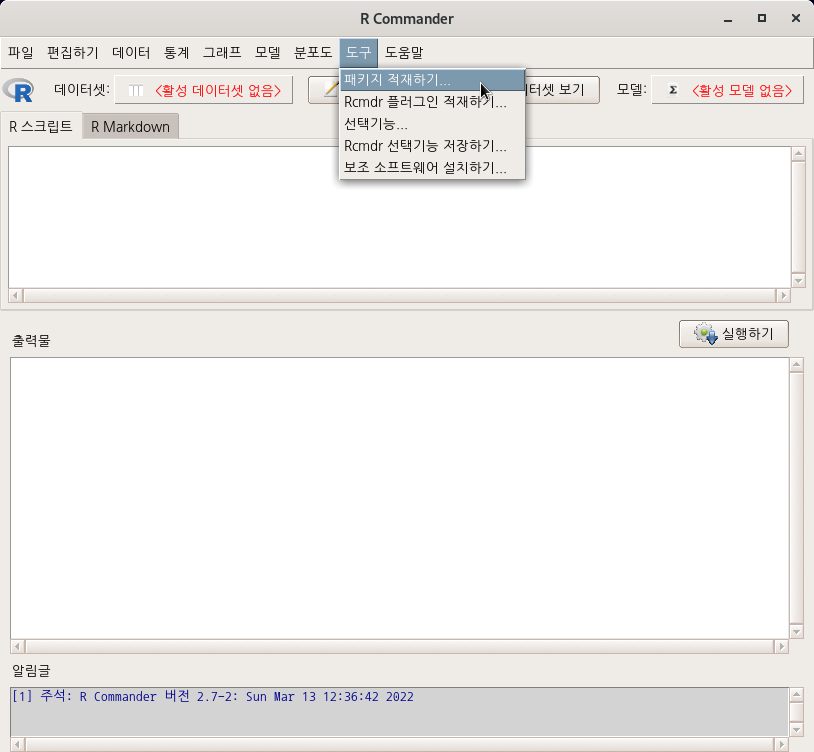
\includegraphics{fig/tools-load-pkg-01.png}

R에 설치된 패키지 목록 창이 등장한다. 원하는 패키지(들)을 찾아서 선택하고 예(OK) 버튼을 누른다. 아래 화면은 vcd 패키지를 설치하는 사례이다.

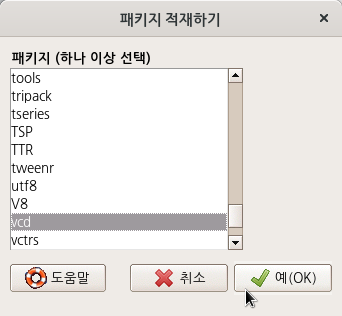
\includegraphics{fig/tools-load-pkg-02.png}

\begin{Shaded}
\begin{Highlighting}[]
\FunctionTok{library}\NormalTok{(vcd) }\CommentTok{\# 원하는 패키지 적재하기}
\end{Highlighting}
\end{Shaded}

\texttt{vcd} 패키지를 적재(loading) 하는데, \texttt{grid} 패키지가 함께 탑재된 것을 출력창에서 확인할 수 있다.
\texttt{grid}는 \texttt{vcd} 패키지가 제작되는데 의존한 패키지임을 의미한다.
어느 패키지가 메모리에 적재되는 과정은 그 패키지가 의존하는 패키지의 자동적인 적재를 동반한다.

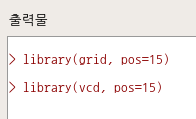
\includegraphics{fig/tools-load-pkg-03.png}

\hypertarget{uxb3c4uxad6c-rcmdr-uxd50cuxb7ecuxadf8uxc778-uxc801uxc7acuxd558uxae30}{%
\section{도구 \textgreater{} Rcmdr 플러그인 적재하기\ldots{}}\label{uxb3c4uxad6c-rcmdr-uxd50cuxb7ecuxadf8uxc778-uxc801uxc7acuxd558uxae30}}

\texttt{도구\ \textgreater{}\ Rcmdr\ 플러그인\ 적재하기...\ /\ Tools\ \textgreater{}\ Load\ Rcmdr\ plug-in(s)....}

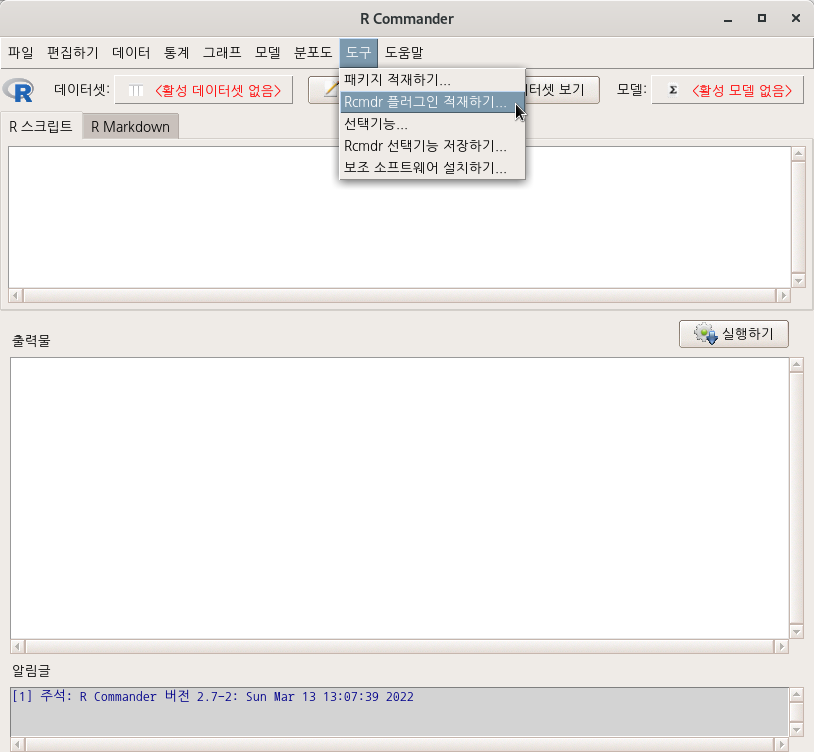
\includegraphics{fig/tools-load-plugin-01.png}

R Commander는 플러그인을 통하여 많은 기능이 확산되는 생태계를 갖고 있다. Rcmdr 플러그인을 사용하기 위해서는 먼저 RcmdrPlugin.이름 을 가진 패키지가 설치되어 있어야 한다.

\begin{Shaded}
\begin{Highlighting}[]
\FunctionTok{install.packages}\NormalTok{()  }\CommentTok{\# RcmdrPlugin.이름 찾기}
\end{Highlighting}
\end{Shaded}

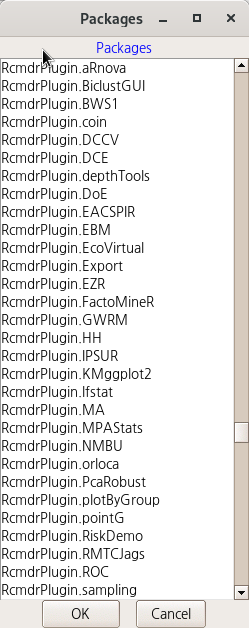
\includegraphics{fig/tools-load-plugin-02.png}

아래와 같이 여러개의 RcmdrPlugin.이름을 가진 플러그인들이 설치되었다고 가정하자. 그 중에서 RcmdrPlugin.KMggplot2를 설치해보자. 적재할 플러그인을 찾아서 선택하고, 예(OK) 버튼을 누른다.

\begin{figure}
\centering
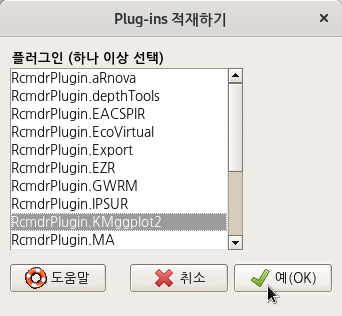
\includegraphics{fig/tools-load-plugin-03.png}
\caption{Linux 사례 (MX 21)}
\end{figure}

Linux 사례 (MX 21)
아래 화면은 플러그인이 적재되기 이전에 새로운 환경이 등장하는 조건을 환기시키는 질문을 담고 있다. R Commander가 사라졌다가 다시 등장하게된다.

\begin{figure}
\centering
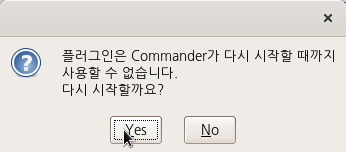
\includegraphics{fig/tools-load-plugin-04.png}
\caption{Linux 사례 (MX 21)}
\end{figure}

새롭게 등장하는 R Commander 화면 상단을 살펴보자. 와 사이에 메뉴 하나가 추가됨을 알 수 있다. 적재된 플러그인이 메뉴 창에 등장한다.

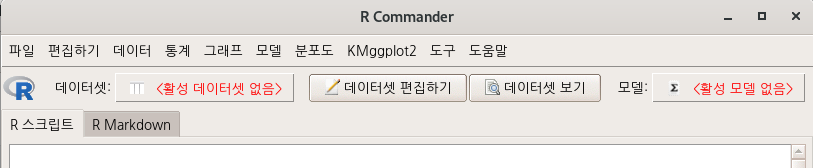
\includegraphics{fig/tools-load-plugin-05.png}

\hypertarget{uxb3c4uxad6c-uxc120uxd0dd-uxae30uxb2a5}{%
\section{도구 \textgreater{} 선택 기능\ldots{}}\label{uxb3c4uxad6c-uxc120uxd0dd-uxae30uxb2a5}}

\texttt{도구\ \textgreater{}\ 선택\ 기능...\ /\ Tools\ \textgreater{}\ Options...}

\begin{figure}
\centering
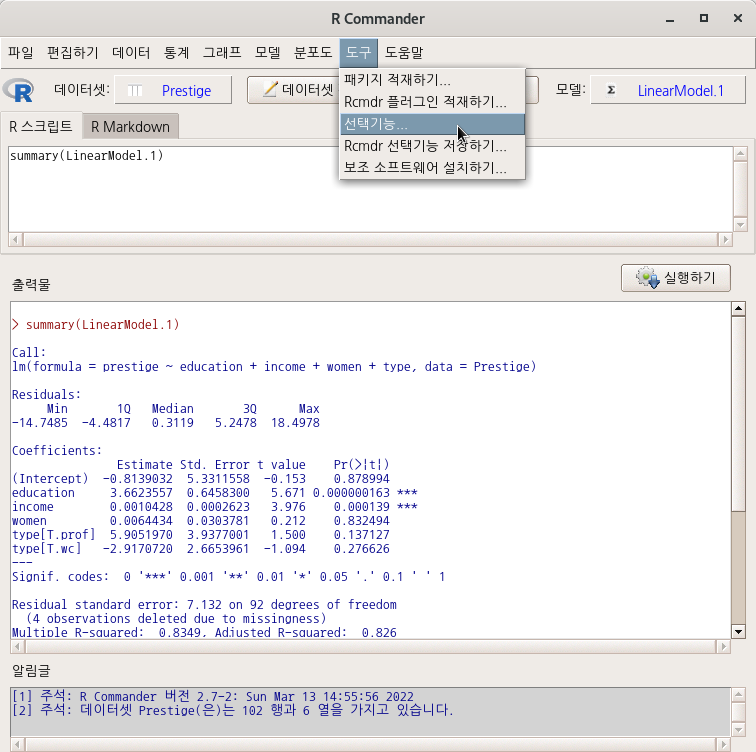
\includegraphics{fig/tools-options-01.png}
\caption{Linux 사례 (MX 21)}
\end{figure}

창에서 스크립트 창 높이 (줄)과 출력물 창 높이 (줄) 을 조정할 수 있다. 자주 R Commander를 사용하다보면, 하나의 명령문을 실행한 다음 얻게되는 출력물을 출력창에서 한번에 보지 못할 때 불편함을 느낀다. 주로 통계적 모델의 요약 정보를 확인하고자 할 때 발생하는 현상이다.

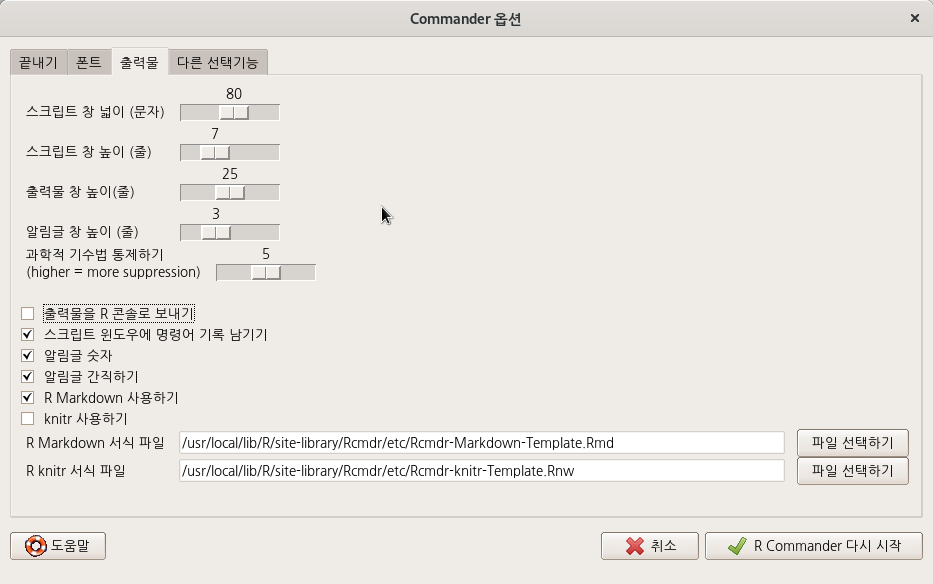
\includegraphics{fig/tools-options-02.png}

아래 창은 스크립트 창 높이 (줄)을 7로, 출력물 창 높이 (줄)을 25로 변경한 사례이다.

\begin{figure}
\centering
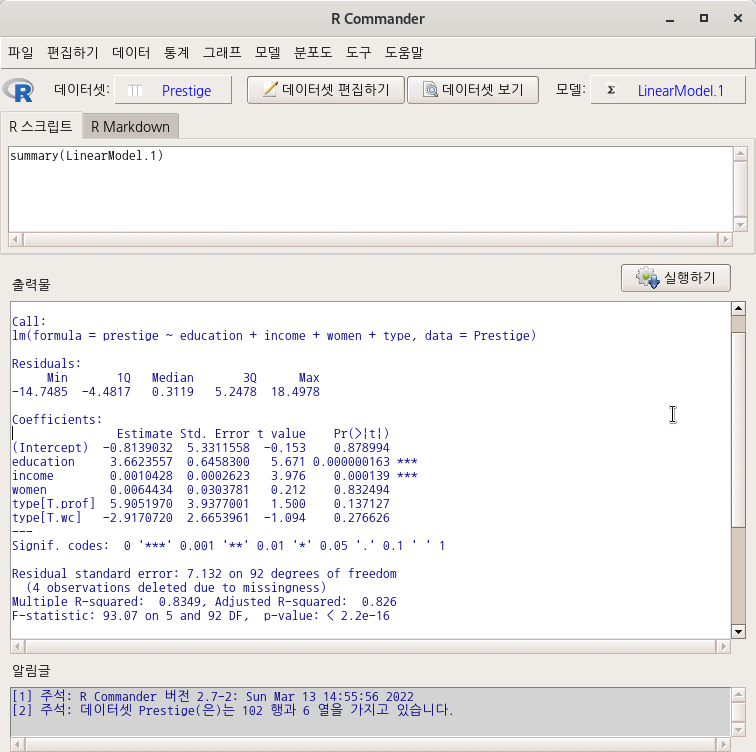
\includegraphics{fig/tools-options-03.png}
\caption{Linux 사례 (MX 21)}
\end{figure}

스크립트 창과 출력 창의 높이를 조정한 결과는 아래와 같은 비율로 나타난다:

\hypertarget{uxae00uxaf34fonts}{%
\section{글꼴(Fonts)}\label{uxae00uxaf34fonts}}

R은 사용 컴퓨터에 내장된 여러 폰트를 사용할 수 있다. R Commander에서 폰트를 고민할 때는 그래프 출력에 어떤 폰트를 사용할까와 화면 출력용으로 어떤 폰트가 좋을까 등일 것이다.

R Commander에는 , 등의 버튼이 화면 상단에 있다. 활성데이터셋의 내부를 들여다 볼 때, 편집할 때 사용한다. 그런데 간혹 사전에 기본으로 지정된 폰트의 특징 때문에 데이터셋의 내부 정보들의 형식적 일관성(값의 정렬)이 흐트러져 보이는 경우가 있다. 예를 들어, 리눅스에서 한글용으로 사용하는 나눔고딕은 한글 R Commander환경에서 기본 폰트로 사용되는데 버튼을 누르고 내부 정보를 보면 정렬이 일정하지 않는 것을 알 수 있다. 흔히 고정크기를 가진 폰트인가 아닌가에 따른 출력상의 차이라고 한다.

사례 값들의 정렬이 일정하지 않아 데이터셋 내부를 보기가 불편하다면, 경험적으로 나는 Courier로 바꿔준다. 일정한 정렬로 변환될 것이다.

\hypertarget{toolssave-rcmdr-options}{%
\section{Tools/Save Rcmdr options\ldots{}}\label{toolssave-rcmdr-options}}

\hypertarget{toolsmanage-mac-os-x-app-nap-for-r.app}{%
\section{Tools/Manage Mac OS X app nap for R.app\ldots{}}\label{toolsmanage-mac-os-x-app-nap-for-r.app}}

\hypertarget{toolsinstall-auxiliary-software}{%
\section{Tools/Install auxiliary software\ldots{}}\label{toolsinstall-auxiliary-software}}

  \bibliography{book.bib,packages.bib}

\end{document}
